\section{Aufbau des Versuchs}
\begin{figure}[h]
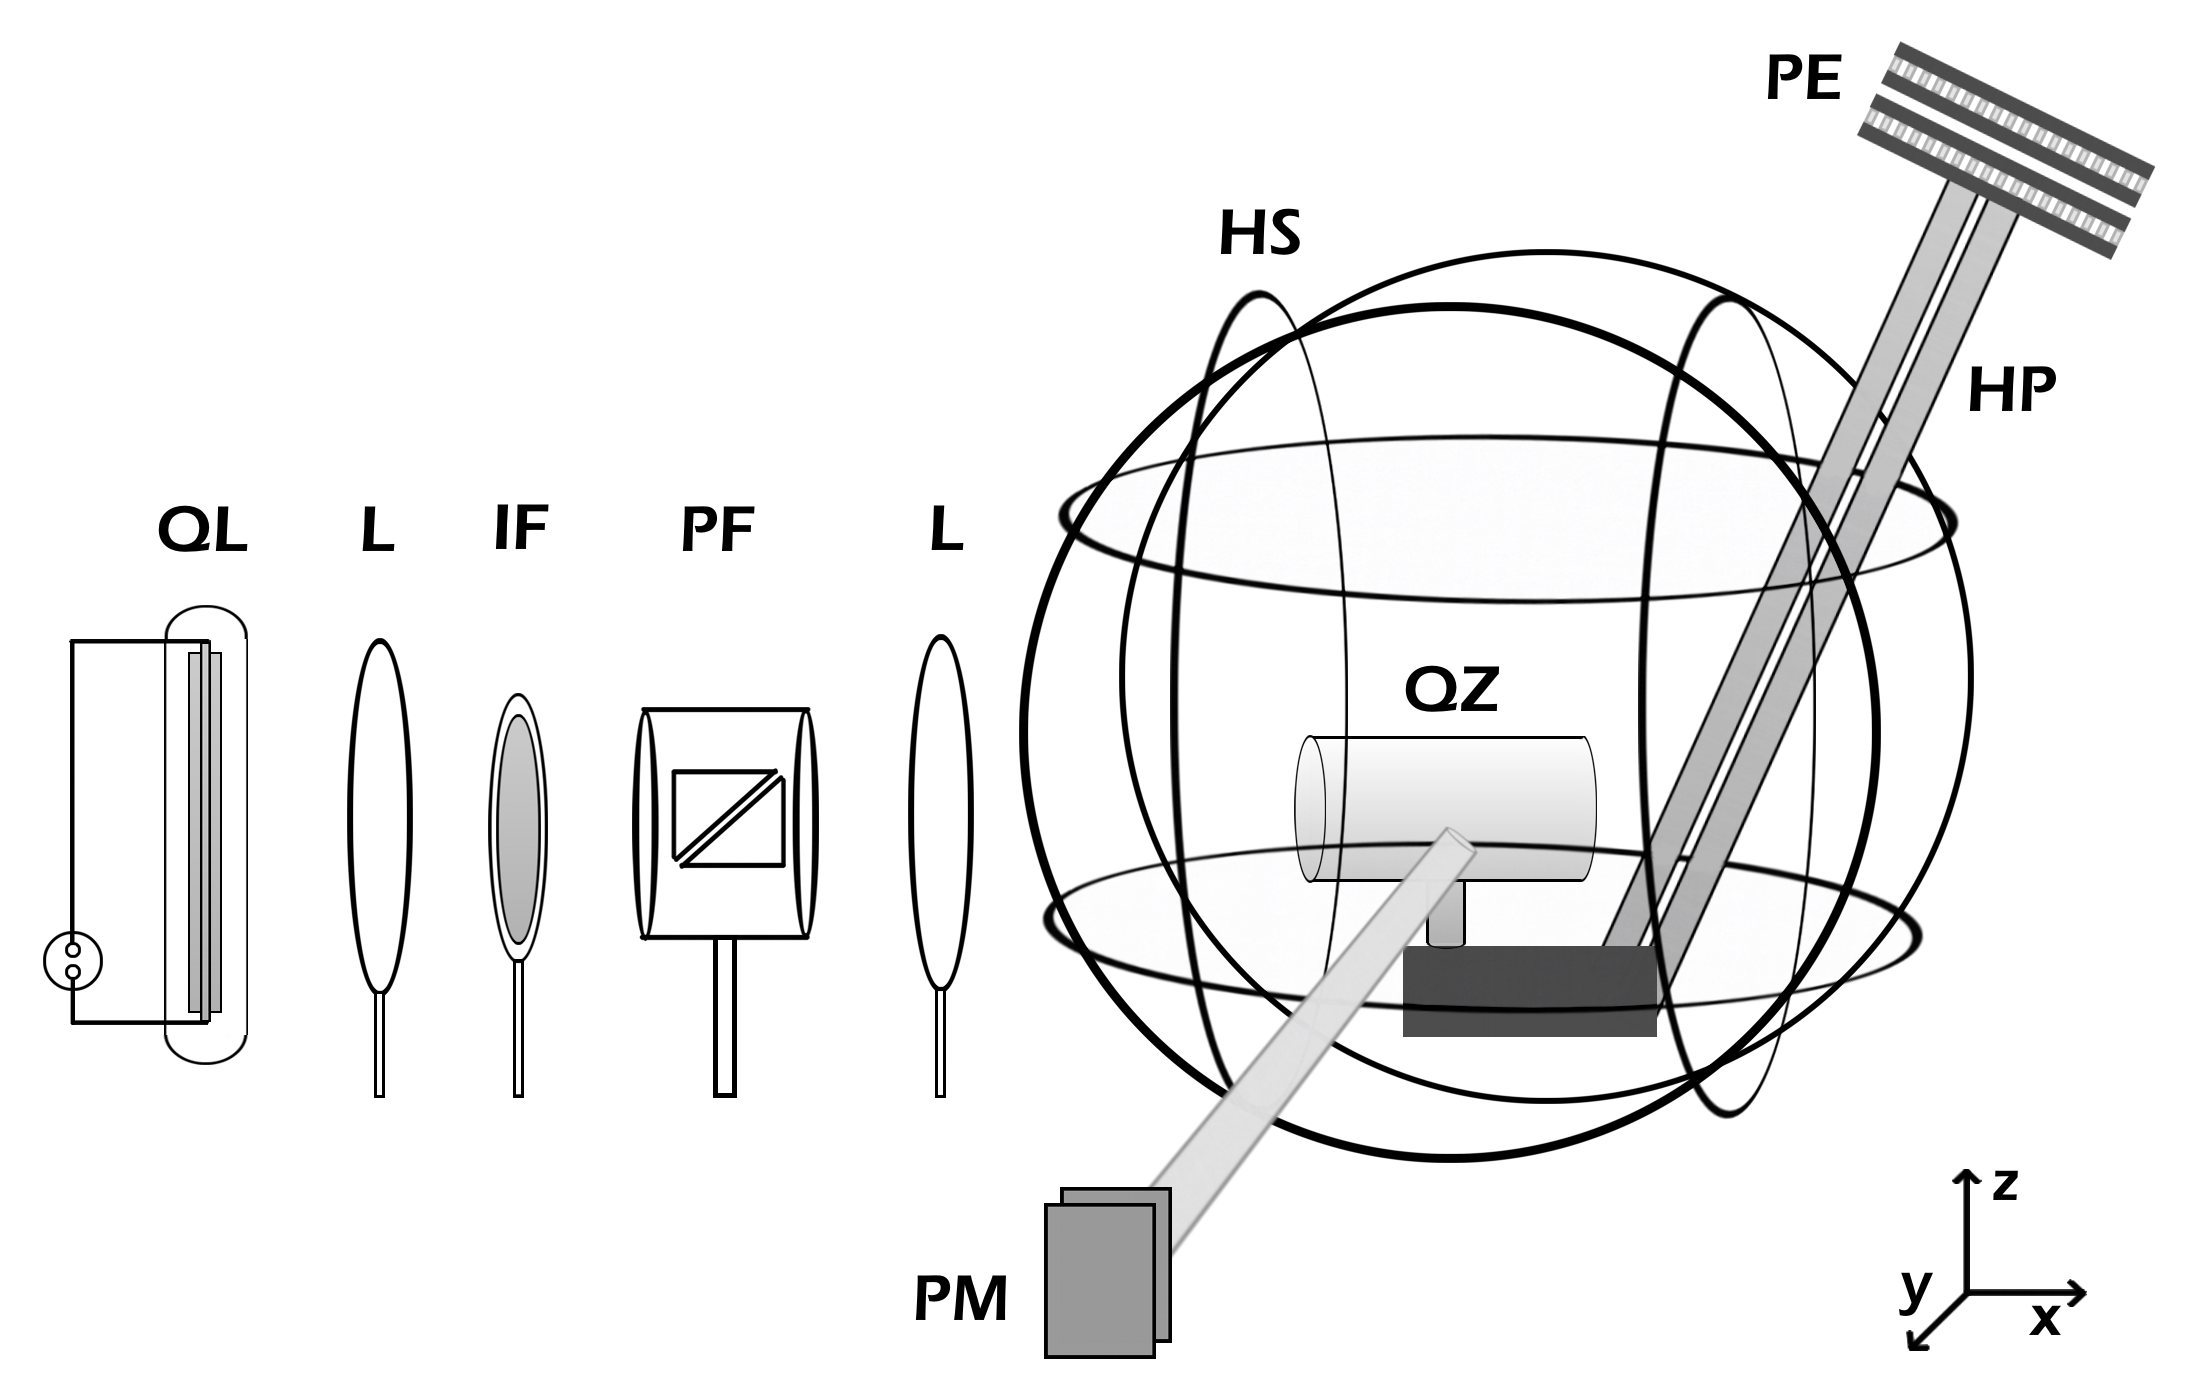
\includegraphics[scale=0.3]{Bilder/aufbau}
\caption{Aufbau. Quelle: [ver]}
\end{figure}
Im Versuch soll die Lebensdauer des durch Licht der Wellenlänge $253,7nm$ angeregten $^{3}P_{1}$-Zustandes von Quecksilber untersucht werden. Dazu benutzt man eine Quecksilberdampf- Niedrigdrucklampe (QL). Das so erzeugte Licht wird von der ersten Linse (L) kollimiert und von der zweiten fokussiert. Zwischen diesen Linsen ist ein Interferenzfilter (IF) angebracht, welche einen Durchlassbereich von $(255\pm5)nm$ FWHM  verwendet und somit die gewünschte Wellenlänge durchlässt. Besonders wichtig ist dabei, dass eine Wellenlänge von $184,5 nm$ herausgefiltert wird, da diese den sonst dominierenden Übergang von Quecksilber zwischen $^{1}P_{1}$ und $^{1}S_{0}$ anregen würde. Ein doppelbrechender Polarisationsfilter (PF) ermöglicht die Wahl der Polarisationsrichtung.\\
Das Licht trifft auf eine Quecksilberdampf-Resonanzzelle (QZ), welche aus einem Quarzkolben und einer Vertiefung im Boden besteht, in welcher sich das Quecksilber sammelt. Zur Kühlung der Zelle werden Peltierlemente (PE) verwendet. Aufgrund ihres elektrischen Störfeldes werden diese mithilfe wärmetransportierender 'Heat Pipes' (HP) möglichst weig weg von der Zelle positioniert. Ebenfalls außerhalb ist ein Photomultiplier (PM) angebracht, welcher über den Photoeffekt das Fluoreszenzlicht in ein elektrisches Signal umwandelt und durch einen Potentialgradienten und mehreren Elektroden das Signal verstärkt.\\
Zur Kompensation von Hintergrund-Magnetfeldern werden zwei Paare von Helmholtz-Spulen (HS) benutzt und ein drittes dient zum Durchfahren des magnetisches Feldes, welches für das Hanle-Signal sorgt.
